\documentclass[a4paper,justified]{tufte-handout}

\usepackage{amsmath,amssymb}
\usepackage{booktabs}
\usepackage{graphicx}
\usepackage{tikz}
\usetikzlibrary{arrows.meta,decorations.pathmorphing,patterns}
\usepackage{xcolor}
\definecolor{accent}{HTML}{A6192E}
\definecolor{ink}{HTML}{222222}
\definecolor{hot}{HTML}{C8102E}
\definecolor{cold}{HTML}{2B5A87}
\graphicspath{{figures/}}

\newcommand{\dd}{\mathrm{d}}
\setlength{\emergencystretch}{1.5em}
\newcommand{\degC}{\,\textdegree{}C}
\newcommand{\lpm}{\,l/min}

\title{Hot water into a cold pipe}
\author{The physics of dead-leg warm-up, and how the deadleg model represents it}
\date{3 October 2026}

\begin{document}
\maketitle

\begin{abstract}
\noindent When a hot tap is opened at the end of a pipe that has gone cold, the
first water out is the cold water that was standing in the pipe. That much is
simple displacement. But the hot water that follows has to heat the pipe wall
as it goes, and it loses a little heat to the air. So the tap runs warm later,
and more water is wasted, than displacement alone suggests. This note sets out
the physics of that transient: the governing equations, the few
dimensionless numbers that control it, the analytical limits, and why copper and
plastic pipes behave so differently. The model built on it predicts the delivery
times of 46 field tests to within a few seconds, with no fitted constants.
\end{abstract}

\section{The question}

Consider a pipe of length $L$ (m) whose bore, the open channel the water flows
through, has radius $r_i$ (m). The pipe holds a volume of water
$V=\pi r_i^2L$ (m$^3$). Let $t$ (s) be the time since the tap was opened, and
$Q$ (m$^3$/s) the volume flow rate through the pipe. If the hot water simply
pushed the cold water out, like a piston, it would reach the tap after the
\emph{plug-flow time}
\begin{equation}
  t_{\text{plug}} = \frac{V}{Q} = \frac{L}{u},
  \qquad u = \frac{Q}{\pi r_i^2},
  \label{eq:plug}
\end{equation}
where $u$ (m/s) is the mean velocity of the water.\sidenote{For 5\,m of
10\,mm copper (bore 8.8\,mm), $V=0.30$\,l, so $t_{\text{plug}}=6$\,s at
3\lpm{} and 18\,s at 1\lpm{}.} The rest of this note explains why the real
delivery time is longer than this, and by how much.

The setting is a domestic hot water branch. Flows are 1 to 6\lpm{}, through
pipes of roughly 10 to 12\,mm outside diameter, made of copper or plastic
(PE-X, cross-linked polyethylene). Before the tap opens, the water in the pipe,
the pipe wall and the surrounding air are all at one starting temperature,
$T_0$ (\textdegree C), typically about 20\degC{}. From $t=0$, water enters the
pipe at the inlet temperature $T_{in}(t)$, for example 55\degC{}.

\section{Four bodies, three exchanges}

\begin{marginfigure}
\centering
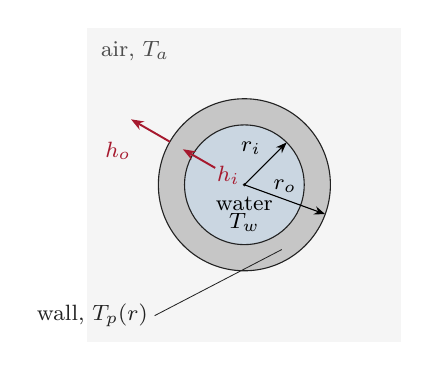
\begin{tikzpicture}[scale=0.95, every node/.style={font=\footnotesize}]
  \fill[gray!8] (-2.1,-2.1) rectangle (2.1,2.1);
  \node[gray!60!black, anchor=north west] at (-2.05,2.05) {air, $T_a$};
  \fill[gray!45] (0,0) circle (1.15);
  \fill[cold!25] (0,0) circle (0.8);
  \draw[ink, line width=0.4pt] (0,0) circle (1.15) (0,0) circle (0.8);
  \node at (0,-0.25) {water};
  \node at (0,-0.5) {$T_w$};
  % radii from the centre
  \fill[ink] (0,0) circle (0.7pt);
  \draw[-{Stealth[length=1.4mm]}, line width=0.4pt] (0,0) -- (45:0.8) node[pos=0.55, above left=-1pt] {$r_i$};
  \draw[-{Stealth[length=1.4mm]}, line width=0.4pt] (0,0) -- (-20:1.15) node[pos=0.5, above=-1pt] {$r_o$};
  % wall label with leader
  \draw[ink, line width=0.3pt] (-60:1.0) -- (-1.2,-1.75) node[left=-1pt] {wall, $T_p(r)$};
  % heat flow, water -> wall -> air
  \draw[accent, -{Stealth[length=1.6mm]}, line width=0.7pt] (150:0.45) -- (150:0.95);
  \node[accent] at (150:0.25) {$h_i$};
  \draw[accent, -{Stealth[length=1.6mm]}, line width=0.7pt] (150:1.15) -- (150:1.75);
  \node[accent] at (165:1.75) {$h_o$};
\end{tikzpicture}
\caption{Cross-section of the pipe. Heat passes from the water to the wall
across the water film (coefficient $h_i$), conducts through the wall, and leaves
its outer surface for the air (coefficient $h_o$). $r_i$ and $r_o$ are the
inner and outer radii.}
\label{fig:section}
\end{marginfigure}

Let $x$ (m) be the distance along the pipe from the inlet, and $r$ (m) the
radial distance from the pipe's axis. The pipe wall occupies $r_i<r<r_o$, where
$r_o$ is the outer radius. The model follows four bodies
(Figure~\ref{fig:section}):
\begin{enumerate}
  \item \textbf{the water}, flowing along the pipe as a plug. Its
    \emph{bulk} temperature $T_w(x,t)$ is the flow-weighted average over the
    cross-section, which is the temperature you would measure if you collected
    and mixed the water passing $x$;
  \item \textbf{the pipe wall}, homogeneous and axially symmetric, with a
    temperature $T_p(r,x,t)$ that varies through the thickness and along the
    length (subscript $p$ for \emph{pipe});
  \item \textbf{the air}, a single well-mixed body at temperature $T_a(t)$ that
    warms as the pipe gives it heat;
  \item optionally, \textbf{an environment}, such as the building fabric, at a
    fixed temperature $T_{env}$, to which the air body can lose heat.
\end{enumerate}
They exchange heat in a chain. Heat passes from the water to the wall by forced
convection, through the wall by conduction, and from the wall to the air by
natural convection and radiation. A \emph{heat transfer coefficient}
(W/m$^2$K) is the heat flow per unit of surface area per degree of temperature
difference. The coefficient between the water and the inner surface of the wall
is $h_i$; the coefficient between the outer surface and the air is $h_o$.
The section on heat transfer coefficients, below, says how both are found.

\section{Governing equations}

\paragraph{Water.} Let $\rho_w$ (kg/m$^3$) and $c_w$ (J/kg\,K) be the density
and specific heat capacity of water, and $A_i=\pi r_i^2$ (m$^2$) the
cross-sectional area of the bore. An energy balance on a thin slice of water,
of length $\dd x$, carried along with the flow gives
\begin{equation}
  \rho_w c_w A_i\left(\frac{\partial T_w}{\partial t}+u\frac{\partial T_w}{\partial x}\right)
  = h_i\, 2\pi r_i\,\bigl(T_p(r_i,x,t)-T_w\bigr).
  \label{eq:water}
\end{equation}
The left side is the rate at which the slice's heat content changes, per metre
of pipe, as seen by an observer moving with the water. The right side is the
heat flowing into the slice from the wall, per metre: the coefficient $h_i$,
times the wetted perimeter $2\pi r_i$, times the difference between the wall's
inner-surface temperature $T_p(r_i,x,t)$ and the water temperature. The inlet
condition is $T_w(0,t)=T_{in}(t)$, and the initial condition is
$T_w(x,0)=T_0$.\sidenote{Two simplifications are made here. First, heat
conduction along the water is neglected. The Péclet number
$Pe=uL/\alpha_w$, the ratio of heat carried by the flow to heat conducted along
it, is about $10^7$; here $\alpha_w=k_w/(\rho_w c_w)$ is the thermal
diffusivity of water and $k_w$ (W/m\,K) its thermal conductivity. Second,
$\rho_w c_w$ is held constant, at its value for the mean of $T_0$ and $T_{in}$,
so that heat is carried along exactly. It varies by less than 1\,\% over this
range.}

\paragraph{Wall.} Let $\rho_p$, $c_p$ and $k_p$ be the density, specific heat
capacity and thermal conductivity of the pipe material.\sidenote{Here $c_p$
means the specific heat of the \emph{pipe} material, not the specific heat at
constant pressure.} Heat conduction in an axially symmetric annulus obeys
\begin{equation}
  \rho_p c_p \frac{\partial T_p}{\partial t}
  = \frac{1}{r}\frac{\partial}{\partial r}\!\left(k_p r \frac{\partial T_p}{\partial r}\right)
  + k_p\frac{\partial^2 T_p}{\partial x^2},
  \qquad r_i<r<r_o .
  \label{eq:wall}
\end{equation}
The first term on the right is conduction through the thickness; the second is
conduction along the pipe. The heat flux leaving a surface by conduction,
$-k_p\,\partial T_p/\partial r$ (W/m$^2$), must equal the flux arriving there by
convection, so the two faces obey
\begin{align}
  -k_p\frac{\partial T_p}{\partial r}\Big|_{r=r_i} &= h_i\bigl(T_w-T_p(r_i)\bigr), \\
  -k_p\frac{\partial T_p}{\partial r}\Big|_{r=r_o} &= h_o\bigl(T_p(r_o)-T_a\bigr).
\end{align}
The wall starts at $T_0$. Its ends, $x=0$ and $x=L$, are treated as insulated.

\paragraph{Air.} Let $\rho_a$ and $c_a$ be the density and specific heat
capacity of air, and $V_a$ (m$^3$) the volume of the air body. Let $UA_{env}$
(W/K) be the conductance between the air body and the environment: the heat
flow per degree of temperature difference, which is zero by default. Because
the air has a single temperature, its energy balance is an ordinary
differential equation:
\begin{equation}
  \rho_a c_a V_a \frac{\dd T_a}{\dd t}
  = \int_0^L h_o\,2\pi r_o\bigl(T_p(r_o,x,t)-T_a\bigr)\,\dd x \;-\; UA_{env}\bigl(T_a-T_{env}\bigr).
  \label{eq:air}
\end{equation}
The integral is the heat arriving from the whole outer surface of the pipe,
which has perimeter $2\pi r_o$. The air starts at $T_a(0)=T_0$. Letting
$V_a\to\infty$ holds the air at $T_0$, which represents a large
room.\sidenote{$c_a$ is the specific heat at constant pressure,
1006\,J/kg\,K. That is appropriate for a void that is not airtight, where the
warming air can expand. For a sealed void the specific heat at constant volume,
about 0.72 times this, would apply instead.}

\paragraph{Conservation.} Let $T_{out}(t)=T_w(L,t)$ be the temperature of the
water leaving at the tap. Measure each body's heat content (J) from the starting
temperature, so that each starts at zero:
\begin{align*}
  E_{\text{water}} &= \int_0^L\rho_w c_w A_i\,(T_w-T_0)\,\dd x,\\
  E_{\text{wall}}  &= \int_0^L\!\!\int_{r_i}^{r_o}\rho_p c_p\,(T_p-T_0)\,2\pi r\,\dd r\,\dd x,\\
  E_{\text{air}}   &= \rho_a c_a V_a\,(T_a-T_0).
\end{align*} Adding equations
\eqref{eq:water}--\eqref{eq:air} and integrating from $0$ to $t$ gives
\begin{multline}
  \int_0^t \rho_w c_w Q\,\bigl(T_{in}-T_{out}\bigr)\,\dd t'
  = E_{\text{water}}+E_{\text{wall}}+E_{\text{air}} \\
  + \int_0^t UA_{env}\bigl(T_a-T_{env}\bigr)\,\dd t' ,
\end{multline}
where $t'$ is the variable of integration. In words: the heat that entered and
has not left at the tap is now in the water, the wall or the air, or has gone
to the environment. The numerical solution satisfies this budget to rounding
error.

\section{What controls the delay}

Writing equations \eqref{eq:water}--\eqref{eq:air} in dimensionless form shows
that three dimensionless groups do almost all the work.

\paragraph{The heat capacity ratio.} Let $A_p=\pi(r_o^2-r_i^2)$ (m$^2$) be the
cross-sectional area of the wall. The ratio
\begin{equation}
  \sigma = \frac{\rho_p c_p A_p}{\rho_w c_w A_i}
\end{equation}
is the heat one metre of wall absorbs per degree of warming, divided by the
heat one metre of water gives up per degree. Suppose the wall took up heat
instantly and nothing was lost to the air. For hot water to pass a point, the
pipe there must first be raised to the hot temperature, which takes
$(1+\sigma)$ times the heat held in the water alone. The hot front, the
position where the water changes from cold to hot, would therefore travel at
speed $u/(1+\sigma)$. It would reach the tap at
\begin{equation}
  t_{\text{front}} = (1+\sigma)\,t_{\text{plug}} .
  \label{eq:front}
\end{equation}
This is the most useful single result in this note. Copper's thin wall gives
$\sigma\approx0.2$; plastic's thick wall gives $\sigma\approx0.5$ to 0.6
(Table~\ref{tab:groups}).\sidenote{Per unit volume, copper stores only about
1.7 times as much heat per degree as PE-X ($\rho_pc_p$ of 3.4 against
2.0\,MJ/m$^3$K). The difference in $\sigma$ comes from the walls: a PE-X wall is
2.5 to 3.3 times as thick, and it surrounds a smaller bore.}

\paragraph{The number of transfer units.} The group
\begin{equation}
  NTU = \frac{h_i\,2\pi r_i L}{\rho_w c_w Q}
\end{equation}
is the heat-exchange capacity of the whole inner surface, in W/K, divided by
the heat capacity flow of the water, also in W/K. It measures how completely
the water gives its heat to the wall in one pass. If it were very large, the
water and the inner surface of the wall would be at the same temperature
everywhere. Over 5\,m of these pipes it is between about 1 and 4. That is large
enough for the wall to take most of the heat from the leading water. It is also
small enough that some slightly warmed water arrives at the plug-flow time, ahead
of the main rise. Above about 2\lpm{}, $NTU$ hardly changes with flow, because
$h_i$ rises almost in proportion to $u$.

\paragraph{The wall Biot number and diffusion time.} Let $\delta=r_o-r_i$ be
the wall thickness and $\alpha_p=k_p/(\rho_p c_p)$ (m$^2$/s) the thermal
diffusivity of the wall material. Then
\begin{equation}
  Bi = \frac{h_i\,\delta}{k_p},\qquad t_{\text{wall}}=\frac{\delta^2}{\alpha_p}.
\end{equation}
The Biot number $Bi$ is the wall's resistance to conduction through its
thickness, $\delta/k_p$, divided by the water film's resistance, $1/h_i$. The
diffusion time $t_{\text{wall}}$ is roughly how long heat takes to soak through
the thickness of the wall. This is where copper and plastic part company:
\begin{itemize}
  \item copper: $Bi\sim0.01$ and $t_{\text{wall}}\approx4$\,ms. The wall is at
    one temperature through its thickness almost as soon as the water touches
    it, so it behaves as a simple lumped heat store;
  \item PE-X: $Bi\sim10$ to 60 and $t_{\text{wall}}\approx12$ to 20\,s. The
    wall is a poor conductor; while the hot water passes, only a thin inner skin
    warms.
\end{itemize}

\begin{table}[h]
\centering
\footnotesize
\begin{tabular}{@{}lrrrrrr@{}}
\toprule
 & bore & $\sigma$ & $t_{\text{wall}}$ & \multicolumn{3}{c}{$NTU$ / $Bi$ at} \\
 \cmidrule(l){5-7}
 & mm & & s & 1\lpm{} & 3\lpm{} & 6\lpm{} \\
\midrule
Copper 10$\times$0.6 & 8.8 & 0.24 & 0.004 & 2.1 / 0.002 & 3.4 / 0.009 & 3.2 / 0.02 \\
Copper 12$\times$0.6 & 10.8 & 0.19 & 0.004 & 1.3 / 0.001 & 2.8 / 0.006 & 2.7 / 0.01 \\
PE-X 10$\times$1.5 & 7.0 & 0.50 & 11.7 & 3.2 / 8 & 4.2 / 31 & 3.9 / 57 \\
PE-X 12$\times$2.0 & 8.0 & 0.59 & 20.8 & 2.5 / 7 & 3.7 / 33 & 3.4 / 60 \\
\bottomrule
\end{tabular}
\caption{The controlling groups for a 5\,m run. Pipes are named by outside
diameter $\times$ wall thickness, in mm. Water properties are taken at
40\degC{}, and $NTU$ is for the whole 5\,m. Copper wall: $k_p=340$\,W/m\,K,
$\rho_pc_p=3.4$\,MJ/m$^3$K. PE-X: $k_p=0.38$\,W/m\,K,
$\rho_pc_p=2.0$\,MJ/m$^3$K.}
\label{tab:groups}
\end{table}

\begin{figure}
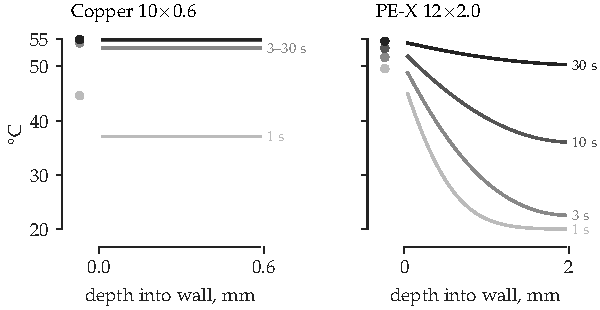
\includegraphics[width=\linewidth]{radial_profiles.pdf}
\caption{Temperature through the wall, half-way along a 5\,m run at 3\lpm{}, at
1, 3, 10 and 30\,s after the hot front passes. The dots at the left are the
water. Copper is uniform through its thickness and catches up with the water in
a few seconds. In PE-X a steep gradient persists: after 10\,s the outer surface
has warmed by only 16\,K, while the water is 33\,K above its starting
temperature.}
\label{fig:radial}
\end{figure}

Figure~\ref{fig:radial} shows the consequence. Copper absorbs its full share of
heat at once, so the outlet stays cool for longer, and its rise is centred near
the delayed front time of equation~\eqref{eq:front}. PE-X takes only a skin of
heat at first. Its \emph{effective} $\sigma$, meaning the part of the wall that
has had time to warm, is small early on and grows as heat penetrates. So the
first warm water arrives close to the plug-flow time, but the last few degrees
wait for the wall to soak through.

\section{Heat transfer coefficients}
\label{sec:htc}

\paragraph{Inside.} The inside coefficient is found from three dimensionless
numbers of the water: the Reynolds number $Re=uD_i/\nu_w$, the Prandtl number
$Pr=\mu_w c_w/k_w$ and the Nusselt number $Nu=h_iD_i/k_w$. Here $D_i=2r_i$ is
the bore diameter, $\mu_w$ (Pa\,s) is the dynamic viscosity of water, and
$\nu_w=\mu_w/\rho_w$ (m$^2$/s) its kinematic viscosity. $Re$ compares inertia
with viscosity and decides whether the flow is laminar or turbulent. $Pr$
compares how fast momentum and heat diffuse. $Nu$ is the heat transfer
coefficient in dimensionless form. For fully turbulent flow, $Re\ge10^4$, the
model uses Gnielinski's correlation,
\begin{equation}
  Nu_{G} = \frac{(f/8)(Re-1000)Pr}{1+12.7\sqrt{f/8}\,(Pr^{2/3}-1)},
  \qquad f=(0.790\ln Re-1.64)^{-2},
\end{equation}
where $f$ is the Darcy friction factor of a smooth pipe. For laminar flow,
$Re\le2300$, it uses $Nu=3.66$, the value for fully developed laminar flow with
a uniform wall temperature. Between the two, it interpolates as the VDI Heat
Atlas recommends:
$Nu=(1-\gamma)\,3.66+\gamma\,Nu_G(10^4)$. Here $Nu_G(10^4)$ is Gnielinski's
value at $Re=10^4$, and the weight is $\gamma=(Re-2300)/(10^4-2300)$.\sidenote{At 1--6\lpm{} in 7--11\,mm bores, $Re$
is about 3000--28000 at 40\degC{}, so the flow is transitional at the lowest
flows and turbulent otherwise. The viscosity of water halves between 20 and
55\degC{}, so the arriving hot water is more turbulent than the cold water it
displaces. The model therefore evaluates $\mu_w$, $k_w$ and $Pr$ at the local
water temperature.} This gives $h_i$ of about $10^3$ to
$1.5\times10^4$\,W/m$^2$K.

\paragraph{Outside.} Let $T_s=T_p(r_o)$ be the outer surface temperature and
$D_o=2r_o$ the outside diameter. The outside coefficient is the sum of a
convective part and a radiative part, $h_o=h_{conv}+h_{rad}$. The convective
part is natural convection from a horizontal cylinder, from the correlation of
Churchill and Chu:
\begin{gather}
  \frac{h_{conv}D_o}{k_a}
  = \left\{0.60+\frac{0.387\,Ra^{1/6}}{\bigl[1+(0.559/Pr_a)^{9/16}\bigr]^{8/27}}\right\}^{2},\\
  Ra=\frac{g\beta\,|T_s-T_a|\,D_o^3}{\nu_a\alpha_a}.
\end{gather}
Here $Ra$ is the Rayleigh number, which measures the strength of buoyancy-driven
flow. $g$ is the acceleration due to gravity, and $\beta$ (1/K) the
expansion coefficient of air, taken as $1/T$ in kelvin. $k_a$, $\nu_a$,
$\alpha_a$ and $Pr_a$ are the conductivity, kinematic viscosity, diffusivity and
Prandtl number of air, at the mean of $T_s$ and $T_a$. The radiative part treats
the surroundings as a large enclosure at the air temperature:
\begin{equation}
  h_{rad}=\varepsilon\,\sigma_{SB}\,(T_s^2+T_a^2)(T_s+T_a),
\end{equation}
with temperatures in kelvin. $\varepsilon$ is the emissivity of the outer
surface and $\sigma_{SB}=5.67\times10^{-8}$\,W/m$^2$K$^4$ the Stefan--Boltzmann
constant. For a 50\degC{} pipe in 20\degC{} air, this gives
$h_o\approx9$\,W/m$^2$K for tarnished copper ($\varepsilon=0.1$) and
$\approx14$\,W/m$^2$K for plastic ($\varepsilon=0.9$).

The outside coefficient is 100 to 1000 times smaller than the inside one. While
the tap runs, a warm pipe loses of the order of 10\,W per metre to the air. The
wall, meanwhile, absorbs heat at hundreds of watts per metre while the front
passes. Over a draw of a minute or two, almost all of the heat leaving the water
goes into the wall. External losses set the steady outlet temperature and how
quickly the pipe cools between draws, but they barely change the delivery time.
The model confirms this. Enclosing the pipe in a 1.5\,m$\times$0.3\,m air body,
instead of holding the air at a fixed temperature, changes no field-trial
prediction by more than 0.34\,s, even though the air warms by up to 7\,K.

\section{Exact solutions in limiting cases}

Three limits have closed-form solutions. Each one checks the model and sharpens
intuition.

\paragraph{No wall heat capacity.} If $\rho_pc_p=0$ and no heat is lost, the
outlet steps from $T_0$ to $T_{in}$ at $t_{\text{plug}}$,
equation~\eqref{eq:plug}.

\paragraph{A thin, perfectly conducting wall with no losses.} If $k_p$ is so
large that the wall is uniform through its thickness, and $h_o=0$, the problem
is the Anzelius--Schumann problem of regenerator theory. Define the
dimensionless water temperature $\theta=(T_w-T_0)/(T_{in}-T_0)$, which runs
from 0 (cold) to 1 (as hot as the supply). Let $P=2\pi r_i$ be the wetted
perimeter, and define the dimensionless distance and time
\[
  \xi = \frac{h_i P x}{\rho_w c_w Q},\qquad
  \eta = \frac{h_i P\,(t-x/u)}{\rho_p c_p A_p}.
\]
$\xi$ is the number of transfer units between the inlet and $x$. $\eta$ is the
time elapsed since the plug-flow front passed $x$, measured in units of the
wall's thermal response time. For a step change in the inlet temperature at
$t=0$, and for $\eta\ge0$,
\begin{equation}
  \theta = e^{-\xi}\Bigl[e^{-\eta}I_0\bigl(2\sqrt{\xi\eta}\bigr)
           +\int_0^\eta e^{-s}I_0\bigl(2\sqrt{\xi s}\bigr)\,\dd s\Bigr].
\end{equation}
For $\eta<0$, that is before the plug front arrives, $\theta=0$. Here $I_0$ is
the modified Bessel function of the first kind, of order zero, and $s$ is a
variable of integration. At the tap, $x=L$, so $\xi$ equals the $NTU$. At the
moment the plug front arrives, $\eta=0$, the bracket equals one. The outlet
therefore jumps to $\theta=e^{-NTU}$: a small step of slightly warmed water.
The rest of the rise is spread around $t_{\text{front}}$ of
equation~\eqref{eq:front}.

\begin{marginfigure}
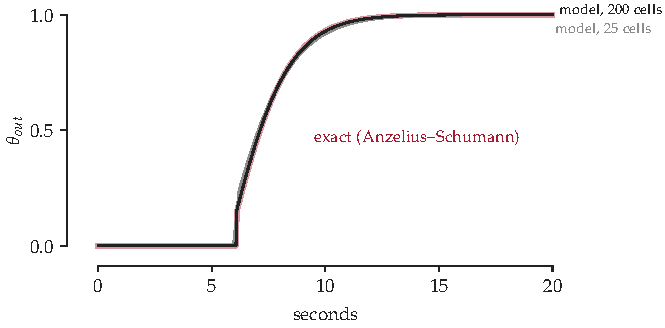
\includegraphics[width=\linewidth]{schumann.pdf}
\caption{The numerical model (grey and black) against the exact
Anzelius--Schumann solution (red), for a copper-like wall, 5\,m at 3\lpm{}.
$\theta_{out}$ is $\theta$ at the tap. Even with 25 cells the curves are almost
indistinguishable.}
\label{fig:schumann}
\end{marginfigure}

\paragraph{Steady state with losses.} After the wall has warmed fully, with the
air at a fixed temperature, the outlet settles at
\begin{gather}
  T_{out} = T_a + (T_{in}-T_a)\exp\!\left(-\frac{U'L}{\rho_w c_w Q}\right),\\
  \frac{1}{U'} = \frac{1}{2\pi r_i h_i}+\frac{\ln(r_o/r_i)}{2\pi k_p}+\frac{1}{2\pi r_o h_o}.
\end{gather}
$U'$ (W/m\,K) is the overall conductance from water to air per metre of pipe:
the inverse of the three resistances in series, namely the water film, the wall
and the outside surface. Because $h_o$ is small, the steady drop over 5\,m is a
fraction of a degree.

\section{How the equations are solved}

The pipe is divided into $N_x$ cells of length $\Delta x=L/N_x$ (200 cells by
default). Each cell has one water temperature and $N_r$ concentric wall shells
of equal thickness, each with its own temperature. There is one air
temperature. Each time step, of length $\Delta t$, does three things:
\begin{enumerate}
  \item \textbf{Radial heat exchange} between the water, the wall shells and the
    air, solved implicitly (backward Euler). In each cell the water and wall
    unknowns form a tridiagonal system, and its solution is linear in the new
    air temperature. That lets the air, which couples every cell, be solved
    exactly in one step, with no iteration;
  \item \textbf{Axial conduction} along the wall, also implicit;
  \item \textbf{Advection}, meaning transport by the flow: the time step is
    chosen as $\Delta t=\Delta x/u$, so the water moves exactly one cell per
    step. Transport is therefore exact, and the front is not artificially
    smeared.
\end{enumerate}
The scheme conserves energy to rounding error. It converges to the
Anzelius--Schumann solution at first order, meaning the error halves when the
number of cells doubles. The largest error is 0.7\,\% with 200 cells and
0.2\,\% with 800 (Figure~\ref{fig:schumann}).

\section{What the model predicts}

\begin{figure}
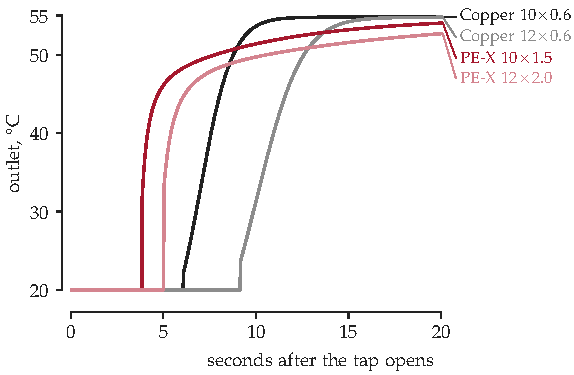
\includegraphics[width=\linewidth]{outlet_traces.pdf}
\caption{Outlet temperature after the tap opens: 5\,m run, 3\lpm{}, inlet
55\degC{}, pipe and air initially 20\degC{}.}
\label{fig:traces}
\end{figure}

Figure~\ref{fig:traces} shows both behaviours. Each copper trace stays at
$T_0$ until $t_{\text{plug}}$ and shows the small step of slightly warmed
water. It then rises steadily over a few seconds, through
$(1+\sigma)\,t_{\text{plug}}$. The PE-X traces jump most of the way towards
40\degC{} at the plug-flow time, then creep towards the inlet temperature as
heat soaks into the wall.

Three practical consequences follow.
\begin{itemize}
  \item \textbf{For copper, the waste is a fixed volume.} About 1.4 to 1.5 pipe
    volumes run off before the tap reaches 50\degC{}, whatever the flow. The
    time therefore scales as $1/Q$.
  \item \textbf{For plastic, the answer depends on what ``hot'' means.} The time
    to 50\degC{} can be twice the time to 40\degC{}. At 1\lpm{}, a PE-X pipe is
    as slow to 50\degC{} as a copper pipe of the same outside diameter, despite
    holding less water. At 6\lpm{} it is faster.
  \item \textbf{A delivery time means something only with its threshold and
    supply temperature.} A 45\degC{} target with a 50\degC{} supply falls in the
    slow tail for plastic pipe.
\end{itemize}

\section{Checking against a field trial}

\begin{marginfigure}
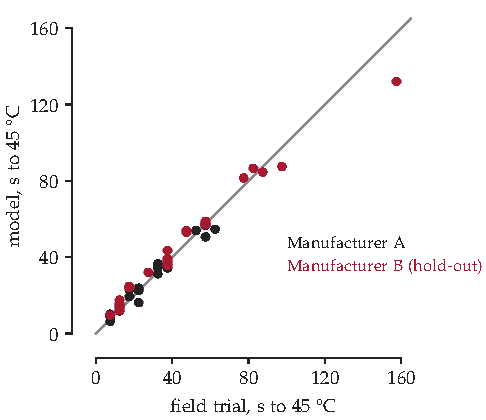
\includegraphics[width=\linewidth]{parity.pdf}
\caption{Model against measured time to 45\degC{} for all 46 field tests. The
diagonal is perfect agreement. Each dot sits half-way through its 5\,s reading
window, and the short horizontal bar spans the window.}
\label{fig:parity}
\end{marginfigure}

Ridge and Jones (FairHeat, 2022) measured the time for the tap to reach
45\degC{}. They tested 5, 15 and 25\,m runs of multilayer pipe (plastic with an
aluminium layer) at 4, 6 and 9\lpm{}. Hot water came from a heat interface
unit, the heat exchanger that serves a flat on a heat network, and the pipe
started at about 19\degC{}. The probe was read every 5\,s. The model was run for
every test with no adjustment. The inlet temperature stepped from 19 to
50\degC{} at the time the unit alone had taken to deliver hot water, which the
paper measured separately. The multilayer wall was represented as one
homogenised material, and the air body was an enclosed 1.5\,m$\times$0.3\,m
cross-section running the length of the pipe.

\begin{table}[h]
\centering
\footnotesize
\begin{tabular}{@{}lrrrr@{}}
\toprule
 & \multicolumn{2}{c}{model} & \multicolumn{2}{c}{paper's regression} \\
 \cmidrule(lr){2-3}\cmidrule(l){4-5}
 & bias & RMS & bias & RMS \\
\midrule
Manufacturer A (23 tests) & $-0.1$\,s & 3.3\,s & $+3.1$\,s & 4.3\,s \\
Manufacturer B, hold-out (23) & $+1.1$\,s & 7.0\,s & $+6.2$\,s & 8.9\,s \\
\bottomrule
\end{tabular}
\caption{Bias is the mean of predicted minus measured time. RMS is the
root-mean-square error. Errors are taken against the middle of each 5\,s
reading window. The paper's regression was fitted to Manufacturer A, so
Manufacturer B is a hold-out set that neither method has seen.}
\label{tab:errors}
\end{table}

The physical model does better than the paper's regression on both sets,
including the set the regression was fitted to (Table~\ref{tab:errors},
Figure~\ref{fig:parity}). Its largest misses are on the slow, long, large-bore
runs at 4\lpm{}, where it predicts hot water 10 to 28\,s early. The likeliest
explanation, which has not yet been tested, is that the heat unit supplied
water a little below 50\degC{} at that flow. Because 45\degC{} is close to the
supply temperature, one degree makes a large difference there.

\section{Limitations}

\begin{itemize}
  \item \textbf{Plug flow.} Below $Re\approx2300$ the flow is laminar. Its
    velocity profile is parabolic, so water on the axis moves at twice the mean
    velocity. The first warm water then arrives at about half the plug-flow
    time, and the front is smeared. This matters only near or below 1\lpm{},
    with cold water.
  \item \textbf{Steady correlations.} A coefficient $h_i$ derived for steady
    conditions is applied to a strongly transient wall. The entrance region and
    the moving thermal front both raise the true coefficient slightly.
  \item \textbf{A homogeneous wall.} Multilayer pipe is represented by
    volume-averaged properties.
  \item \textbf{What is left out.} Fittings, clips, insulation and the thermal
    mass of the surrounding structure are not modelled. Radiation is taken to
    go to surroundings at the air temperature.
\end{itemize}

\vspace{1em}
\noindent{\footnotesize\raggedright The code, tests and data behind this note are in the
GitHub repository \mbox{gwilma/deadleg\_deadtime}. The file
\mbox{docs/derivation.md} gives the same derivation in brief, and
\mbox{docs/physics/make\_figures.py} redraws every figure.\par}

\end{document}
